% ============================================================
% Capítulo 00: Os Fundamentos do Pensamento de Engenharia
% ============================================================
\chapter{Os Fundamentos do Pensamento de Engenharia}

\section{Introdução}

O que diferencia um engenheiro de software de alguém que apenas escreve código? A resposta não está na linguagem de programação dominada, no framework da moda ou na velocidade com que se digita. Está na forma de \textbf{pensar}. A engenharia de software é, antes de tudo, uma disciplina do pensamento --- uma maneira estruturada de abordar problemas complexos, antecipar consequências e tomar decisões sob incerteza.

Vivemos uma era em que modelos de linguagem de grande escala (LLMs) podem gerar código funcional em segundos. O GitHub Copilot, o ChatGPT e ferramentas similares transformaram a escrita de código em algo cada vez mais automatizável. Diante dessa realidade, surge uma pergunta inevitável: qual é o papel do engenheiro de software quando a máquina já sabe programar? A resposta está justamente nos fundamentos que este capítulo apresenta. A inteligência artificial já escreve código que funciona. O diferencial humano é \textbf{saber qual código escrever} --- e, talvez mais importante, qual código \textbf{não} escrever.

Um programador resolve o problema imediato. Quando o código compila e os testes passam, a tarefa está concluída. Um engenheiro, por outro lado, pergunta qual é o \emph{problema real}, quem será afetado pela solução, o que acontece quando o sistema falha às três da manhã de um domingo, e como a decisão de hoje vai reverberar nos próximos dois, cinco ou dez anos. Essa diferença de perspectiva não é um luxo acadêmico --- é o que separa sistemas que prosperam de sistemas que desmoronam sob o peso de suas próprias decisões acumuladas.

\begin{quote}
``A essência da engenharia de software é gerenciar complexidade, não produzi-la.'' --- Grady Booch
\end{quote}

O pensamento sistêmico, a análise de trade-offs, a mentalidade de longo prazo e a responsabilidade ética formam os quatro pilares sobre os quais se constrói a identidade profissional do engenheiro. Cada decisão técnica --- desde a escolha de um banco de dados até a definição de um contrato de API --- afeta o todo. Uma mudança aparentemente inofensiva em um módulo pode provocar falhas em cascata em componentes que, à primeira vista, não possuem relação alguma.

A responsabilidade do engenheiro de software transcende o código. Falhas em sistemas de software já causaram mortes reais. O caso do Therac-25, uma máquina de radioterapia cujo software defeituoso administrou doses letais de radiação a pacientes nos anos 1980, é um lembrete sombrio de que código não é abstração --- é ação no mundo real. O caso do Boeing 737 MAX, cujo software MCAS contribuiu para dois acidentes fatais que mataram 346 pessoas, reforça que decisões de engenharia carregam peso moral.

Este capítulo estabelece os alicerces conceituais que sustentam todo o restante do livro. Antes de falar sobre arquitetura, padrões de design, inteligência artificial ou DevOps, precisamos alinhar a forma como pensamos. Porque ferramentas mudam, linguagens evoluem, frameworks nascem e morrem --- mas os princípios fundamentais do pensamento de engenharia permanecem.

\section{O que é Engenharia de Software}

\subsection{Definição e Escopo}

Engenharia é a aplicação sistemática de princípios científicos e matemáticos para construir algo útil, seguro e confiável. Quando falamos de engenharia de software, estamos aplicando essa mesma disciplina a uma matéria-prima peculiar: o código. Diferente do aço, do concreto ou dos circuitos, o código é intangível, infinitamente maleável e aparentemente sem custo de replicação. Essa natureza cria uma ilusão perigosa: a de que ``consertar depois'' é fácil e barato. Na prática, não é. É apenas mais barato no curtíssimo prazo, acumulando juros compostos de complexidade que eventualmente cobram seu preço.

A engenharia civil não testa o prédio depois de pronto --- calcula antes de construir. Um engenheiro estrutural não ergue vinte andares para ``ver se aguenta''. Ele modela, simula, calcula margens de segurança e só então autoriza a construção. A engenharia de software deveria operar com a mesma disciplina. No entanto, a cultura do ``move fast and break things'' popularizada pelo Vale do Silício normalizou uma abordagem que seria impensável em qualquer outra disciplina de engenharia.

\subsection{O Custo Exponencial da Mudança}

Uma das leis mais bem documentadas da engenharia de software é o crescimento exponencial do custo da mudança ao longo do ciclo de vida de um sistema. Uma decisão de arquitetura equivocada no início de um projeto pode custar centenas de vezes mais para corrigir quando o sistema já está em produção, servindo milhões de usuários.

\begin{table}[h]
\centering
\caption{Custo relativo de correção de defeitos por fase do projeto}
\begin{tabular}{lcc}
\toprule
\textbf{Fase} & \textbf{Custo Relativo} & \textbf{Exemplo} \\
\midrule
Requisitos & 1$\times$ & Ajustar especificação no documento \\
Design & 5$\times$ & Redesenhar módulo antes da implementação \\
Implementação & 10$\times$ & Refatorar código durante o desenvolvimento \\
Testes & 20$\times$ & Corrigir bug encontrado em QA \\
Produção & 100--1000$\times$ & Migrar banco com milhões de registros \\
\bottomrule
\end{tabular}
\label{tab:custo-mudanca}
\end{table}

Esses números, derivados de estudos clássicos de Barry Boehm e confirmados pela experiência da indústria, explicam por que investir tempo em arquitetura e design não é ``perfeccionismo'' --- é economia. O Netflix, por exemplo, investiu anos construindo sua infraestrutura de microsserviços e ferramentas de resiliência como o Chaos Monkey precisamente porque entendeu que o custo de corrigir problemas de escalabilidade em produção seria catastrófico.

\subsection{A Interdisciplinaridade da Engenharia de Software}

A engenharia de software não é uma ilha isolada na ciência da computação. Ela bebe de múltiplas disciplinas, e o engenheiro eficaz é aquele que transita entre elas com fluência:

\begin{itemize}
    \item \textbf{Ciência da Computação}: algoritmos, estruturas de dados, teoria da computação --- as fundações técnicas.
    \item \textbf{Matemática}: lógica formal, estatística, teoria de grafos, álgebra relacional --- a linguagem da precisão.
    \item \textbf{Psicologia Cognitiva}: como humanos leem código, como equipes tomam decisões, por que vieses cognitivos afetam estimativas.
    \item \textbf{Economia}: análise de custo-benefício, teoria dos jogos, incentivos --- toda decisão técnica é também uma decisão econômica.
    \item \textbf{Comunicação}: documentação, diagramas, apresentações --- um sistema que ninguém entende é um sistema que ninguém mantém.
    \item \textbf{Sociologia}: dinâmicas de equipe, cultura organizacional, Lei de Conway --- a estrutura da organização molda a estrutura do software.
\end{itemize}

A Lei de Conway, formulada por Melvin Conway em 1967, afirma que ``organizações que projetam sistemas são inevitavelmente constrangidas a produzir designs que são cópias das estruturas de comunicação dessas organizações''. Em outras palavras, se sua empresa tem três times, seu sistema provavelmente terá três módulos principais. Essa observação, aparentemente trivial, tem implicações profundas: a arquitetura do software é indissociável da arquitetura organizacional.

\section{Modelos Mentais do Engenheiro}

\subsection{O que são Modelos Mentais}

Um modelo mental é uma representação simplificada da realidade que usamos para raciocinar sobre sistemas complexos. Engenheiros de software, conscientemente ou não, operam com dezenas de modelos mentais simultâneos: o modelo de como a memória funciona, o modelo de como o HTTP transporta dados, o modelo de como o usuário interage com a interface. A qualidade das decisões de um engenheiro é diretamente proporcional à qualidade de seus modelos mentais.

\begin{quote}
``Todos os modelos são errados, mas alguns são úteis.'' --- George Box
\end{quote}

Essa frase, originalmente sobre modelos estatísticos, aplica-se perfeitamente à engenharia de software. O diagrama de arquitetura que você desenha no quadro branco é uma simplificação grosseira do sistema real. Mas é essa simplificação que permite raciocinar sobre ele, comunicar decisões e identificar problemas antes que se manifestem em produção.

\subsection{Pensamento por Primeiros Princípios}

O pensamento por primeiros princípios (\emph{first principles thinking}) é uma abordagem que consiste em decompor um problema até suas verdades fundamentais e reconstruir o raciocínio a partir delas, em vez de raciocinar por analogia. Elon Musk popularizou o termo no contexto empresarial, mas a técnica remonta a Aristóteles.

Na engenharia de software, pensar por primeiros princípios significa questionar pressupostos que frequentemente são aceitos sem exame:

\begin{itemize}
    \item ``Precisamos de microsserviços'' --- \emph{Por quê? Qual problema de escalabilidade, deploy ou ownership de equipe justifica a complexidade distribuída?}
    \item ``Vamos usar NoSQL'' --- \emph{Quais são os padrões de acesso? Os dados são realmente não-relacionais, ou estamos evitando aprender SQL?}
    \item ``Precisamos de Kubernetes'' --- \emph{Quantos requests por segundo atendemos? Três containers num Docker Compose não resolveriam?}
\end{itemize}

O pensamento por primeiros princípios é um antídoto contra o \emph{hype-driven development} --- a tendência de adotar tecnologias porque são populares, e não porque resolvem o problema em questão.

\subsection{Níveis de Abstração}

Um dos modelos mentais mais poderosos da engenharia de software é o conceito de \textbf{níveis de abstração}. Todo sistema pode ser observado em diferentes altitudes, e o engenheiro eficaz sabe transitar entre elas com fluidez:

\begin{figure}[htbp]
    \centering
    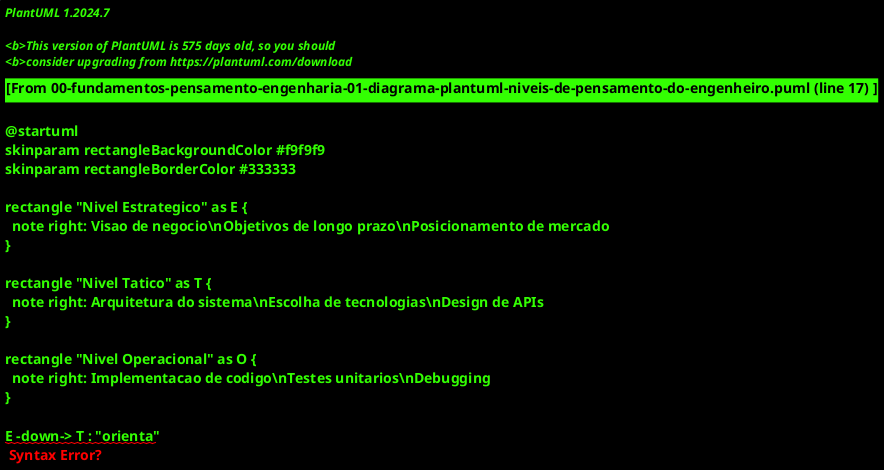
\includegraphics[width=0.85\textwidth]{imagens/00-fundamentos-pensamento-engenharia-01-diagrama-plantuml-niveis-de-pensamento-do-engenheiro.png}
    \caption{Diagrama PlantUML: Níveis de Pensamento do Engenheiro}
\end{figure}

O nível \textbf{estratégico} lida com perguntas como ``qual problema de negócio estamos resolvendo?'' e ``como este sistema se posiciona no ecossistema da empresa?''. O nível \textbf{tático} trata de decisões como ``usaremos uma arquitetura de eventos ou request-response?'' e ``como dividiremos os bounded contexts?''. O nível \textbf{operacional} é onde o código é efetivamente escrito, os testes são executados e os bugs são corrigidos.

O erro mais comum entre desenvolvedores juniores é permanecer exclusivamente no nível operacional, escrevendo código sem entender o contexto tático e estratégico que deveria orientar cada linha. O erro mais comum entre arquitetos seniores é flutuar exclusivamente no nível estratégico, produzindo diagramas elegantes que não sobrevivem ao contato com a realidade do código.

\subsection{A Tabela: Programador vs.\ Engenheiro vs.\ Arquiteto}

Para tornar concreta a diferença entre os modos de pensar, a tabela a seguir compara três perfis frequentemente confundidos na indústria:

\begin{table}[h]
\centering
\caption{Comparação entre Programador, Engenheiro e Arquiteto de Software}
\begin{tabular}{p{3cm}p{3.5cm}p{3.5cm}p{3.5cm}}
\toprule
\textbf{Dimensão} & \textbf{Programador} & \textbf{Engenheiro} & \textbf{Arquiteto} \\
\midrule
Pergunta central & ``Como faço isso funcionar?'' & ``Qual a melhor solução para este contexto?'' & ``Como este sistema evolui nos próximos 5 anos?'' \\
\addlinespace
Horizonte temporal & Horas a dias & Semanas a meses & Meses a anos \\
\addlinespace
Escopo de preocupação & Função ou módulo & Sistema completo & Ecossistema de sistemas \\
\addlinespace
Métrica de sucesso & Funciona corretamente & Funciona, escala e é mantível & Alinhado ao negócio e adaptável \\
\addlinespace
Relação com trade-offs & Desconhece ou ignora & Analisa e documenta & Define os critérios de decisão \\
\addlinespace
Conhecimento chave & Linguagem e frameworks & Design, testes, infra & Domínio de negócio e estratégia \\
\bottomrule
\end{tabular}
\label{tab:programador-engenheiro-arquiteto}
\end{table}

É importante notar que esses perfis não são cargos mutuamente exclusivos. Um engenheiro sênior eficaz transita entre os três modos de pensar conforme a necessidade. A tabela descreve \emph{modos de operação}, não títulos em um crachá.

\section{O Pensamento Sistêmico}

\subsection{Vendo o Todo, Não Apenas as Partes}

Pensamento sistêmico é a capacidade de compreender um sistema como um todo integrado, onde o comportamento emerge das interações entre as partes, e não das partes isoladas. Peter Senge, em \emph{A Quinta Disciplina}, popularizou o conceito no contexto organizacional. Na engenharia de software, o pensamento sistêmico é o que permite ao engenheiro antecipar que uma mudança ``simples'' em um módulo pode provocar efeitos em cascata por todo o sistema.

O sistema não é a soma de suas partes --- é o produto das interações entre elas. Um banco de dados relacional, um servidor de aplicação e uma fila de mensagens são componentes simples quando analisados individualmente. Mas as interações entre eles --- latência de rede, consistência eventual, retentativas, timeouts --- criam comportamentos emergentes que nenhum dos componentes possui isoladamente. É nesses interstícios que a maioria dos bugs graves se esconde.

\subsection{Interdependências e Acoplamento}

No coração do pensamento sistêmico está o conceito de \textbf{interdependência}. O módulo A depende do módulo B, que depende do módulo C, que --- surpresa --- depende do módulo A. Essas dependências circulares são mais comuns do que gostaríamos de admitir, e cada uma delas é um ponto de fragilidade.

\begin{figure}[htbp]
    \centering
    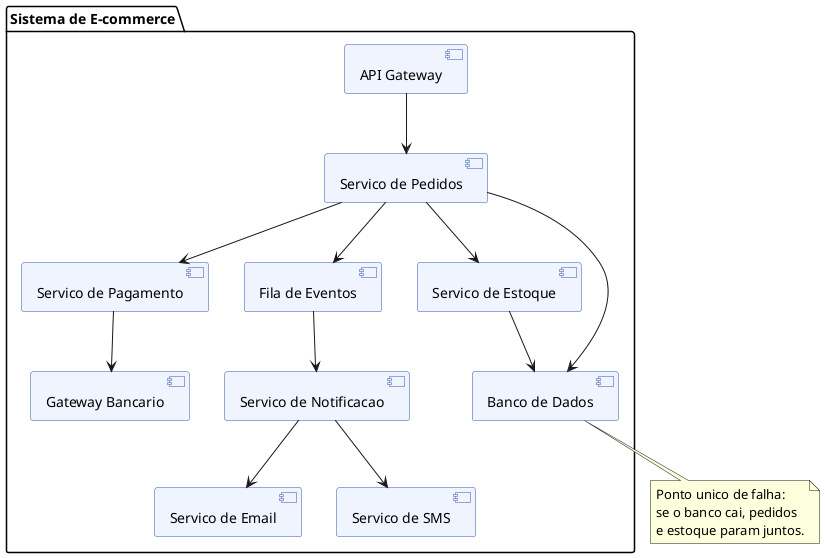
\includegraphics[width=0.85\textwidth]{imagens/00-fundamentos-pensamento-engenharia-02-diagrama-plantuml-dependencias-sistemicas-entre-componentes.png}
    \caption{Diagrama PlantUML: Dependências Sistêmicas entre Componentes}
\end{figure}

O \textbf{acoplamento} é a medida de quanto dois módulos sabem um do outro. Acoplamento forte significa que mudar a implementação interna de um módulo obriga a modificar o outro. Acoplamento fraco significa que módulos interagem por meio de interfaces bem definidas, permitindo que cada um evolua independentemente. O objetivo não é eliminar todo acoplamento --- isso é impossível e indesejável --- mas torná-lo \emph{explícito e gerenciável}.

\subsection{Efeitos de Segunda Ordem}

Um dos conceitos mais importantes do pensamento sistêmico são os \textbf{efeitos de segunda ordem}: as consequências indiretas de uma decisão que não são imediatamente óbvias.

Considere um exemplo concreto: sua aplicação está lenta. A solução óbvia é adicionar uma camada de cache. O efeito de primeira ordem é positivo: as respostas ficam mais rápidas. Mas os efeitos de segunda ordem incluem: dados potencialmente desatualizados servidos ao usuário, complexidade adicional na invalidação do cache, uso de memória que pode impactar outros processos, e uma nova categoria inteira de bugs relacionados a consistência.

Outro exemplo: adicionar um campo ``status'' a uma tabela do banco de dados parece uma mudança inofensiva. Até você descobrir que 47 microsserviços leem essa tabela, que 12 deles fazem queries filtrando por status, e que a adição do novo campo requer migração coordenada em todos eles.

\begin{lstlisting}[language=Python, caption={Exemplo: Cache que introduz complexidade de segunda ordem}]
import time
from functools import lru_cache
from typing import Optional

class ProdutoService:
    """
    Servico de produtos com cache.
    Parece simples, mas esconde armadilhas de segunda ordem.
    """

    @lru_cache(maxsize=1000)
    def buscar_produto(self, produto_id: int) -> dict:
        """
        Efeito de 1a ordem: resposta rapida.
        Efeito de 2a ordem: produto pode ter sido atualizado
        no banco, mas o cache ainda serve dados antigos.
        """
        return self._consultar_banco(produto_id)

    def atualizar_preco(self, produto_id: int, novo_preco: float):
        self._atualizar_banco(produto_id, novo_preco)
        # PERIGO: esquecemos de invalidar o cache!
        # Clientes verao o preco antigo ate o cache expirar.
        # Em producao, isso pode significar vender produtos
        # pelo preco errado durante horas.

    def atualizar_preco_seguro(self, produto_id: int, novo_preco: float):
        self._atualizar_banco(produto_id, novo_preco)
        # Invalidacao explicita do cache
        self.buscar_produto.cache_clear()
        # Mas agora TODOS os produtos perdem o cache,
        # nao apenas o que foi atualizado.
        # Efeito de 3a ordem: pico de carga no banco.

    def _consultar_banco(self, produto_id: int) -> dict:
        # Simulacao de consulta ao banco de dados
        time.sleep(0.1)  # Latencia simulada
        return {"id": produto_id, "nome": "Produto X", "preco": 99.90}

    def _atualizar_banco(self, produto_id: int, novo_preco: float):
        # Simulacao de atualizacao no banco de dados
        pass
\end{lstlisting}

O engenheiro que pensa sistemicamente não se contenta com a solução de primeira ordem. Ele pergunta: ``e o que acontece \emph{depois}?''

\subsection{Ferramentas para o Pensamento Sistêmico}

Para aplicar o pensamento sistêmico na prática, o engenheiro dispõe de diversas ferramentas conceituais e técnicas:

\begin{itemize}
    \item \textbf{Diagramas de dependência}: mapas visuais que mostram quais componentes dependem de quais, revelando pontos únicos de falha e dependências circulares.
    \item \textbf{Matrizes de impacto}: tabelas que cruzam componentes com possíveis mudanças, classificando o impacto de cada combinação.
    \item \textbf{Análise de grafos de componentes}: aplicação de teoria de grafos para identificar componentes com alto grau de acoplamento (\emph{fan-in} e \emph{fan-out}).
    \item \textbf{Diagramas de contexto (C4)}: modelagem hierárquica do sistema em quatro níveis de zoom, do contexto ao código.
    \item \textbf{Mapas de calor de mudanças}: visualização de quais arquivos ou módulos mudam juntos com frequência, revelando acoplamento implícito.
\end{itemize}

\section{Trade-offs: A Essência da Decisão}

\subsection{Não Existe Solução Perfeita}

Se há uma verdade universal na engenharia de software, é esta: \textbf{não existe solução perfeita}. Existe apenas a solução adequada para um determinado contexto, conjunto de restrições e momento no tempo. Toda decisão técnica é um trade-off --- ao ganhar em uma dimensão, necessariamente perdemos em outra.

O Teorema CAP, formulado por Eric Brewer em 2000, é talvez a expressão mais elegante dessa realidade no campo de sistemas distribuídos: é impossível para um sistema distribuído oferecer simultaneamente Consistência, Disponibilidade e Tolerância a Partições. Você pode ter, no máximo, duas dessas três propriedades. Não é uma limitação de implementação --- é uma impossibilidade matemática.

\begin{quote}
``Arquitetura é a arte de tomar decisões que são difíceis de reverter.'' --- Martin Fowler
\end{quote}

\subsection{Os Trade-offs Fundamentais}

A seguir, exploramos os trade-offs mais recorrentes que o engenheiro de software enfrenta ao longo de sua carreira:

\textbf{Performance versus Legibilidade.} Código ultra-otimizado, com truques de bit manipulation e loops desenrolados, pode ser significativamente mais rápido --- mas também significativamente mais difícil de entender e manter. Na vasta maioria dos casos, a legibilidade vence. Como Donald Knuth famosamente declarou: ``a otimização prematura é a raiz de todo mal''. O engenheiro sábio escreve código legível primeiro, mede a performance segundo, e otimiza apenas os pontos que os dados indicam como gargalos reais.

\textbf{Velocidade de entrega versus Qualidade.} Entregar rápido gera dívida técnica. Entregar com perfeição pode significar entregar tarde demais --- quando o mercado já mudou ou o concorrente já lançou. O caso do Knight Capital Group, em 2012, ilustra o extremo perigoso desse trade-off: uma atualização de software mal feita, lançada com pressa, causou um prejuízo de 440 milhões de dólares em apenas 45 minutos, levando a empresa à falência. Por outro lado, empresas que buscam perfeição antes de lançar frequentemente descobrem que construíram o produto errado para um mercado que já não existe.

\textbf{Flexibilidade versus Simplicidade.} Um sistema genérico demais, projetado para atender qualquer caso futuro, é inerentemente complexo. Um sistema simples demais, que atende apenas o caso atual, precisará ser reescrito quando os requisitos mudarem --- e eles sempre mudam. O princípio YAGNI (\emph{You Aren't Gonna Need It}) sugere errar para o lado da simplicidade, adicionando flexibilidade apenas quando a necessidade se manifesta concretamente.

\textbf{Build versus Buy.} Construir internamente oferece controle total, personalização e independência de fornecedores. Comprar ou adotar soluções prontas economiza tempo, reduz risco e permite focar no diferencial competitivo. A Amazon construiu internamente praticamente toda sua infraestrutura e acabou criando a AWS. A maioria das empresas, no entanto, não é a Amazon --- e a decisão de construir um banco de dados próprio quando o PostgreSQL resolve o problema é, na maioria dos contextos, uma demonstração de ego, não de engenharia.

\subsection{O Framework de Análise de Trade-offs}

Para estruturar a análise de trade-offs, o engenheiro pode seguir um processo disciplinado:

\begin{figure}[htbp]
    \centering
    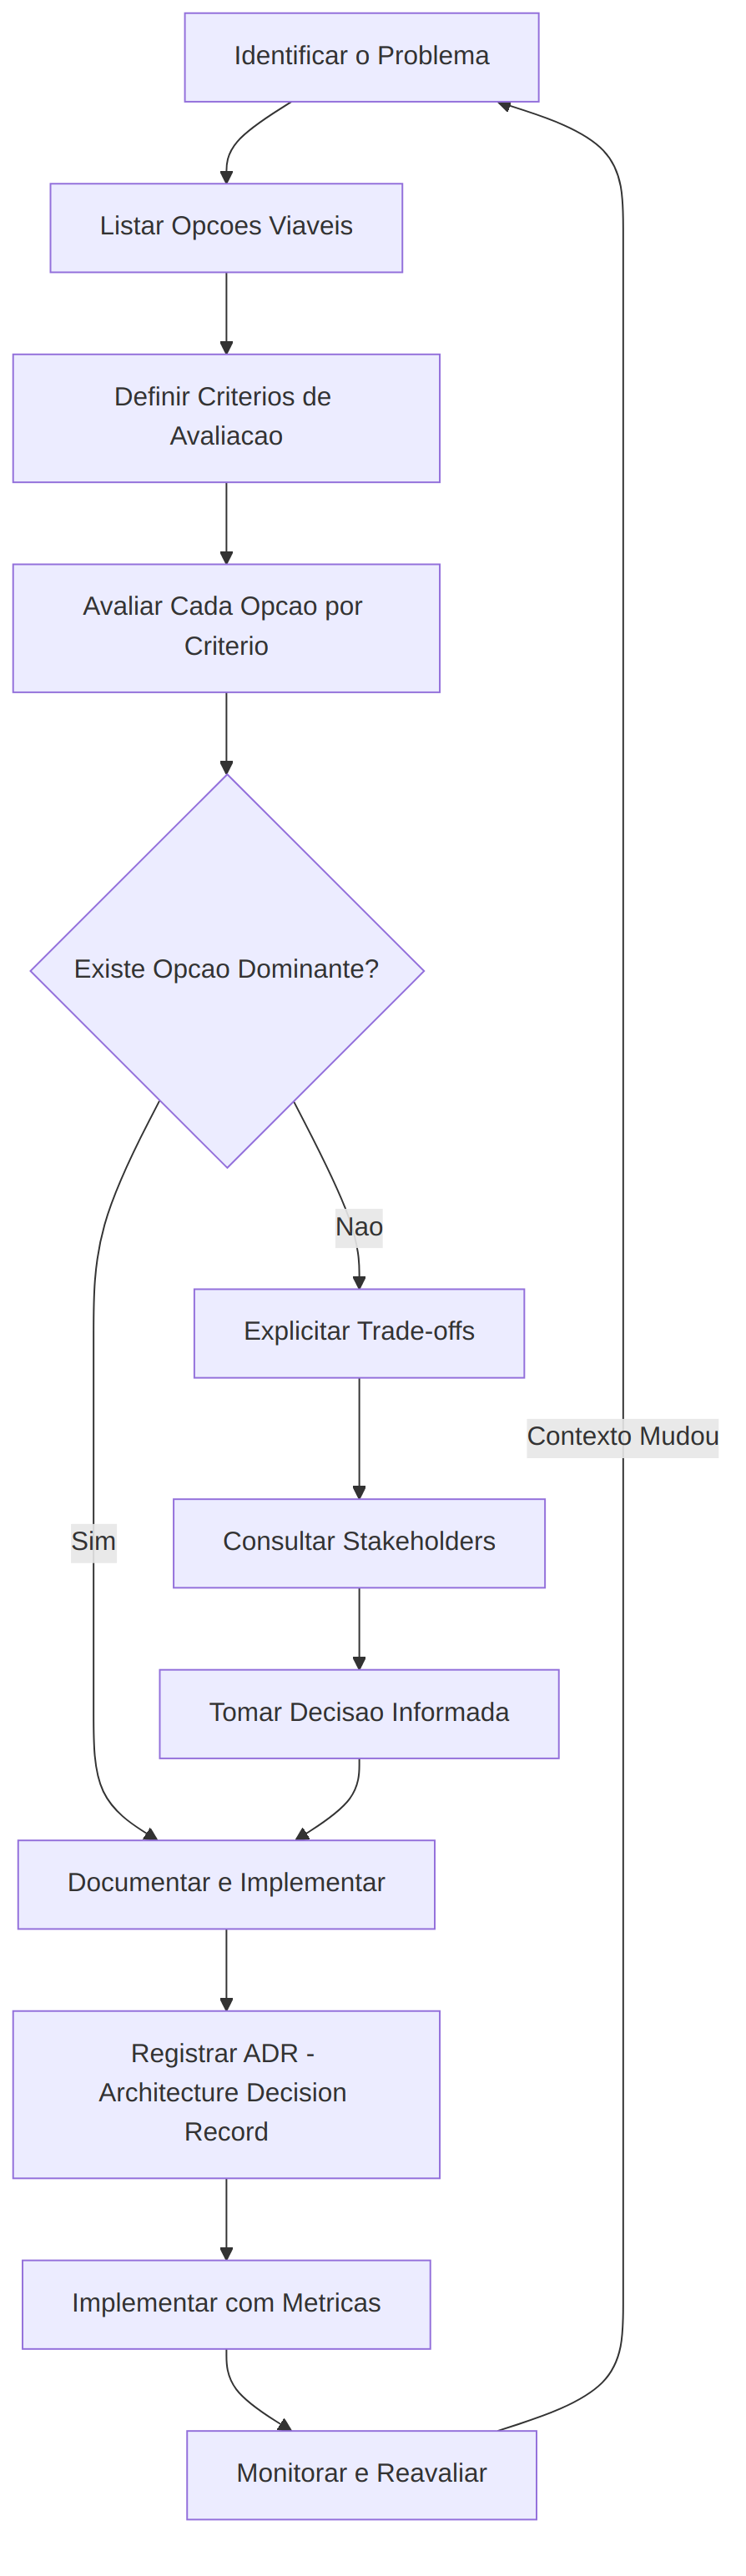
\includegraphics[width=0.85\textwidth]{imagens/00-fundamentos-pensamento-engenharia-03-diagrama-mermaid-framework-de-analise-de-trade-offs.png}
    \caption{Diagrama Mermaid: Framework de Análise de Trade-offs}
\end{figure}

O conceito de \textbf{Architecture Decision Records} (ADRs) é especialmente valioso nesse processo. Um ADR é um documento curto que registra uma decisão de arquitetura, o contexto em que foi tomada, as alternativas consideradas e as razões para a escolha. Meses ou anos depois, quando alguém perguntar ``por que usamos MongoDB em vez de PostgreSQL?'', o ADR terá a resposta --- em vez de depender da memória de alguém que talvez nem trabalhe mais na empresa.

\begin{lstlisting}[language={}, caption={Exemplo de Architecture Decision Record (ADR)}]
# ADR 007: Uso de Fila de Mensagens para Processamento Assincrono

## Status
Aceito

## Contexto
O servico de pedidos processa pagamentos de forma sincrona,
causando timeout quando o gateway bancario demora mais de 5s.
Usuarios veem erro 504 em 3% dos pedidos.

## Decisao
Adotar RabbitMQ para processar pagamentos de forma assincrona.
O pedido sera criado com status "pendente" e confirmado apos
o processamento pela fila.

## Alternativas Consideradas
1. Aumentar timeout para 30s - resolve o sintoma, nao a causa
2. Kafka - excesso de complexidade para o volume atual (500 msg/min)
3. SQS da AWS - lock-in de provedor, time sem experiencia

## Consequencias
- Positivas: resiliencia a falhas do gateway, melhor UX
- Negativas: consistencia eventual, complexidade de monitoramento,
  necessidade de tratar mensagens duplicadas (idempotencia)
\end{lstlisting}

\subsection{A Pergunta de Ouro}

Diante de qualquer decisão técnica, a pergunta mais poderosa que o engenheiro pode fazer é: \textbf{``Qual problema estamos otimizando?''} Essa pergunta simples corta camadas de discussão improdutiva e força a equipe a explicitar suas prioridades. Quando dois engenheiros discordam sobre a melhor abordagem, frequentemente o desacordo não é técnico --- é sobre qual atributo de qualidade priorizar. Um está otimizando para performance, o outro para manutenibilidade. Ambos estão ``certos'' dentro de seu próprio enquadramento. A pergunta de ouro revela o enquadramento e permite uma discussão produtiva.

\section{O Ciclo de Feedback}

\subsection{Build-Measure-Learn para Engenheiros}

O conceito de ciclo de feedback rápido, popularizado por Eric Ries no \emph{Lean Startup}, aplica-se com igual força à engenharia de software. Cada decisão técnica é, em essência, uma hipótese. ``Acreditamos que usar cache Redis reduzirá a latência do P95 de 800ms para 200ms.'' Essa hipótese precisa ser validada com dados, não com opiniões.

O ciclo de feedback do engenheiro opera em múltiplas escalas temporais:

\begin{itemize}
    \item \textbf{Segundos}: o compilador ou linter informa se o código está sintaticamente correto.
    \item \textbf{Minutos}: testes unitários validam se a lógica funciona para os casos conhecidos.
    \item \textbf{Horas}: testes de integração revelam se os componentes interagem corretamente.
    \item \textbf{Dias}: code review por pares identifica problemas de design e legibilidade.
    \item \textbf{Semanas}: métricas de produção mostram se o sistema atende os requisitos não-funcionais.
    \item \textbf{Meses}: indicadores de negócio revelam se a funcionalidade entrega valor real.
\end{itemize}

\begin{figure}[htbp]
    \centering
    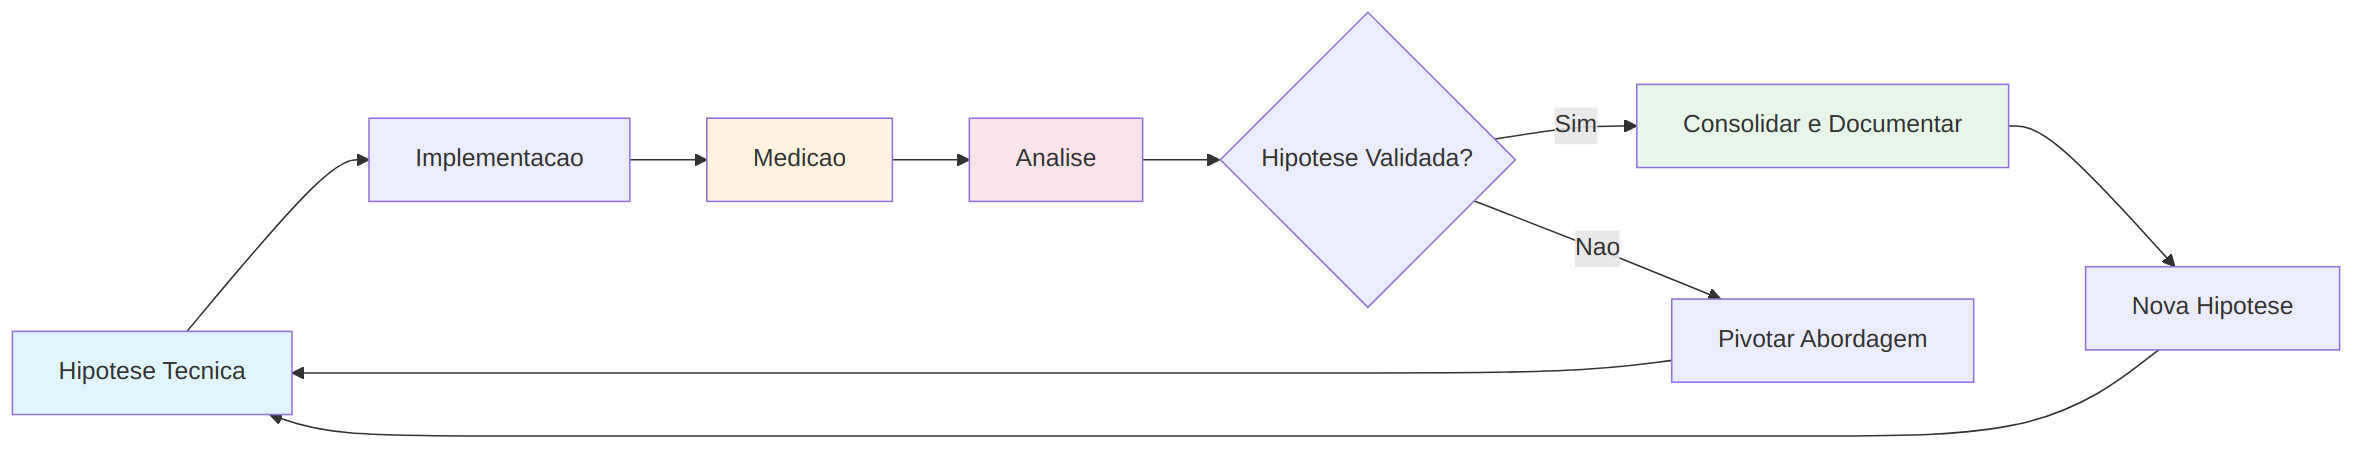
\includegraphics[width=0.85\textwidth]{imagens/00-fundamentos-pensamento-engenharia-04-diagrama-mermaid-o-ciclo-de-feedback-de-decisoes-de-engenhar.png}
    \caption{Diagrama Mermaid: O Ciclo de Feedback de Decisões de Engenharia}
\end{figure}

\subsection{O Perigo do Feedback Ausente}

Quando o ciclo de feedback é longo ou inexistente, decisões ruins se acumulam silenciosamente. Sistemas sem monitoramento adequado são como dirigir à noite com os faróis desligados: tudo parece bem até o momento em que não está mais.

O caso da Amazon em 2012 ilustra o valor do feedback rápido. Um deploy defeituoso no serviço de Elastic Load Balancing provocou uma cascata de falhas que derrubou parte significativa da infraestrutura da AWS na região US-East-1. O que transformou um bug comum em um incidente de proporção catastrófica foi a ausência de mecanismos de rollback automático rápido. Após o incidente, a Amazon investiu pesadamente em sistemas de deploy progressivo (canary deployments) que permitem detectar problemas em segundos, não em horas.

A Netflix, por sua vez, levou o conceito de feedback ao extremo com seu \emph{Chaos Engineering}: a prática deliberada de injetar falhas em produção para testar a resiliência do sistema. O raciocínio é contra-intuitivo mas sólido: se falhas vão acontecer de qualquer forma (e vão), é melhor que aconteçam em condições controladas, quando a equipe está preparada, do que às três da manhã de um feriado.

\subsection{Feedback no Código: Testes como Documentação Viva}

Na escala do código, testes automatizados são a forma mais imediata de feedback. Mas seu valor vai além de ``verificar se funciona''. Testes bem escritos servem como \textbf{documentação viva} das intenções do desenvolvedor:

\begin{lstlisting}[language=Python, caption={Testes como documentação de comportamento esperado}]
import pytest

class TestCalculadoraDeDesconto:
    """
    Estes testes documentam as regras de negocio
    do sistema de descontos, nao apenas a implementacao.
    """

    def test_cliente_novo_nao_recebe_desconto(self):
        calc = CalculadoraDeDesconto()
        desconto = calc.calcular(
            cliente=Cliente(meses_ativo=0),
            valor_compra=100.00
        )
        assert desconto == 0.0

    def test_cliente_fiel_recebe_10_porcento(self):
        """Clientes com mais de 12 meses recebem 10%."""
        calc = CalculadoraDeDesconto()
        desconto = calc.calcular(
            cliente=Cliente(meses_ativo=13),
            valor_compra=100.00
        )
        assert desconto == 10.0

    def test_desconto_maximo_eh_30_porcento(self):
        """
        Independente da antiguidade, o desconto
        nunca ultrapassa 30%. Regra definida pelo
        financeiro em 2024-Q1.
        """
        calc = CalculadoraDeDesconto()
        desconto = calc.calcular(
            cliente=Cliente(meses_ativo=999),
            valor_compra=100.00
        )
        assert desconto <= 30.0
\end{lstlisting}

Observe como os nomes dos testes e os docstrings comunicam \emph{intenção} e \emph{contexto de negócio}, não detalhes de implementação. Quando um teste falha, a mensagem de erro não apenas indica que algo quebrou --- indica \emph{qual regra de negócio} foi violada.

\section{A Mentalidade de Longo Prazo}

\subsection{Código é Lido Mais do que é Escrito}

Uma das verdades mais citadas --- e menos praticadas --- da engenharia de software é que código é lido dez vezes mais do que é escrito. Robert C. Martin, em \emph{Clean Code}, dedica capítulos inteiros a essa ideia. Quando você escreve uma função, está criando algo que será lido, interpretado e possivelmente modificado por dezenas de pessoas ao longo de anos. Investir tempo em legibilidade não é vaidade estética --- é respeito profissional com seus futuros colegas, que talvez incluam você mesmo daqui a seis meses, quando já terá esquecido o que aquele código faz.

\begin{lstlisting}[language=Python, caption={Contraste entre código obscuro e código expressivo}]
# Versao obscura: funciona, mas o que faz?
def proc(d, t):
    return [x for x in d if x['ts'] > t and x['s'] == 'A' and x['v'] > 0]

# Versao expressiva: a mesma logica, legivel
def filtrar_transacoes_ativas_recentes(
    transacoes: list[dict],
    timestamp_minimo: float
) -> list[dict]:
    """
    Retorna transacoes que sao:
    - Mais recentes que o timestamp minimo
    - Com status ativo ('A')
    - Com valor positivo
    """
    return [
        transacao for transacao in transacoes
        if transacao['timestamp'] > timestamp_minimo
        and transacao['status'] == 'A'
        and transacao['valor'] > 0
    ]
\end{lstlisting}

Ambas as funções fazem exatamente a mesma coisa. A diferença é que a segunda pode ser entendida em cinco segundos por qualquer membro da equipe, enquanto a primeira exige que o leitor deduza o significado de cada variável abreviada --- um exercício que consome tempo e introduz risco de interpretação equivocada.

\subsection{Dívida Técnica: Ferramenta, Não Vilã}

O termo ``dívida técnica'', cunhado por Ward Cunningham, é frequentemente usado como sinônimo de ``código ruim''. Mas a metáfora original é mais sutil e mais rica. Dívida técnica é um \textbf{atalho consciente} que acelera a entrega no curto prazo em troca de trabalho futuro --- exatamente como uma dívida financeira. E assim como na vida financeira, o problema não é ter dívida: é não gerenciá-la.

Há momentos em que assumir dívida técnica é a decisão \emph{certa}. Uma startup que precisa validar uma hipótese de mercado em duas semanas não deveria investir três meses construindo uma arquitetura perfeita para um produto que talvez não tenha clientes. O engenheiro maduro sabe assumir dívida técnica deliberadamente, documentá-la explicitamente e pagá-la antes que os juros se tornem insustentáveis.

A dívida técnica se torna perigosa quando é \textbf{involuntária} (resultado de ignorância ou pressa irrefletida) ou \textbf{invisível} (ninguém sabe que existe até o sistema parar). A prática de registrar dívida técnica como itens explícitos no backlog, com estimativas de custo de pagamento, transforma algo abstrato em algo gerenciável.

\subsection{Manutenibilidade e a Regra do Escoteiro}

A manutenibilidade --- a facilidade com que um sistema pode ser modificado para corrigir defeitos, melhorar performance ou adaptar-se a novos requisitos --- é talvez o atributo de qualidade mais subvalorizado na indústria. Sistemas que são fáceis de manter custam menos, evoluem mais rápido e atraem engenheiros melhores (porque ninguém quer trabalhar em um código ilegível e frágil).

A \textbf{Regra do Escoteiro} aplicada ao código é simples e poderosa: ``deixe o código melhor do que você o encontrou''. Cada vez que tocar em um arquivo para fazer uma mudança, aproveite para melhorar um nome de variável, extrair uma constante mágica, adicionar um comentário esclarecedor ou remover um trecho de código morto. Individualmente, essas melhorias são pequenas. Acumuladas ao longo do tempo, transformam um codebase caótico em um codebase habitável.

\subsection{Documentação como Investimento}

Duas horas escrevendo documentação economizam vinte horas explicando a mesma coisa verbalmente para diferentes pessoas ao longo dos próximos meses. Documentação não é burocracia --- é \textbf{alavancagem}. É a forma mais eficiente de multiplicar conhecimento sem exigir a presença física do detentor original da informação.

A documentação mais valiosa não é aquela que descreve \emph{o que} o sistema faz (o código já faz isso), mas aquela que explica \emph{por que} as decisões foram tomadas. Os ADRs mencionados anteriormente são um exemplo perfeito. Outro exemplo são os ``README'' de módulos que explicam o contexto de negócio, as premissas assumidas e os limites conhecidos do componente.

\section{O Processo de Pensamento do Engenheiro}

Para sintetizar os conceitos discutidos até aqui, podemos visualizar o processo completo de pensamento do engenheiro de software como um fluxo estruturado que vai da compreensão do problema até a entrega e monitoramento da solução:

\begin{figure}[htbp]
    \centering
    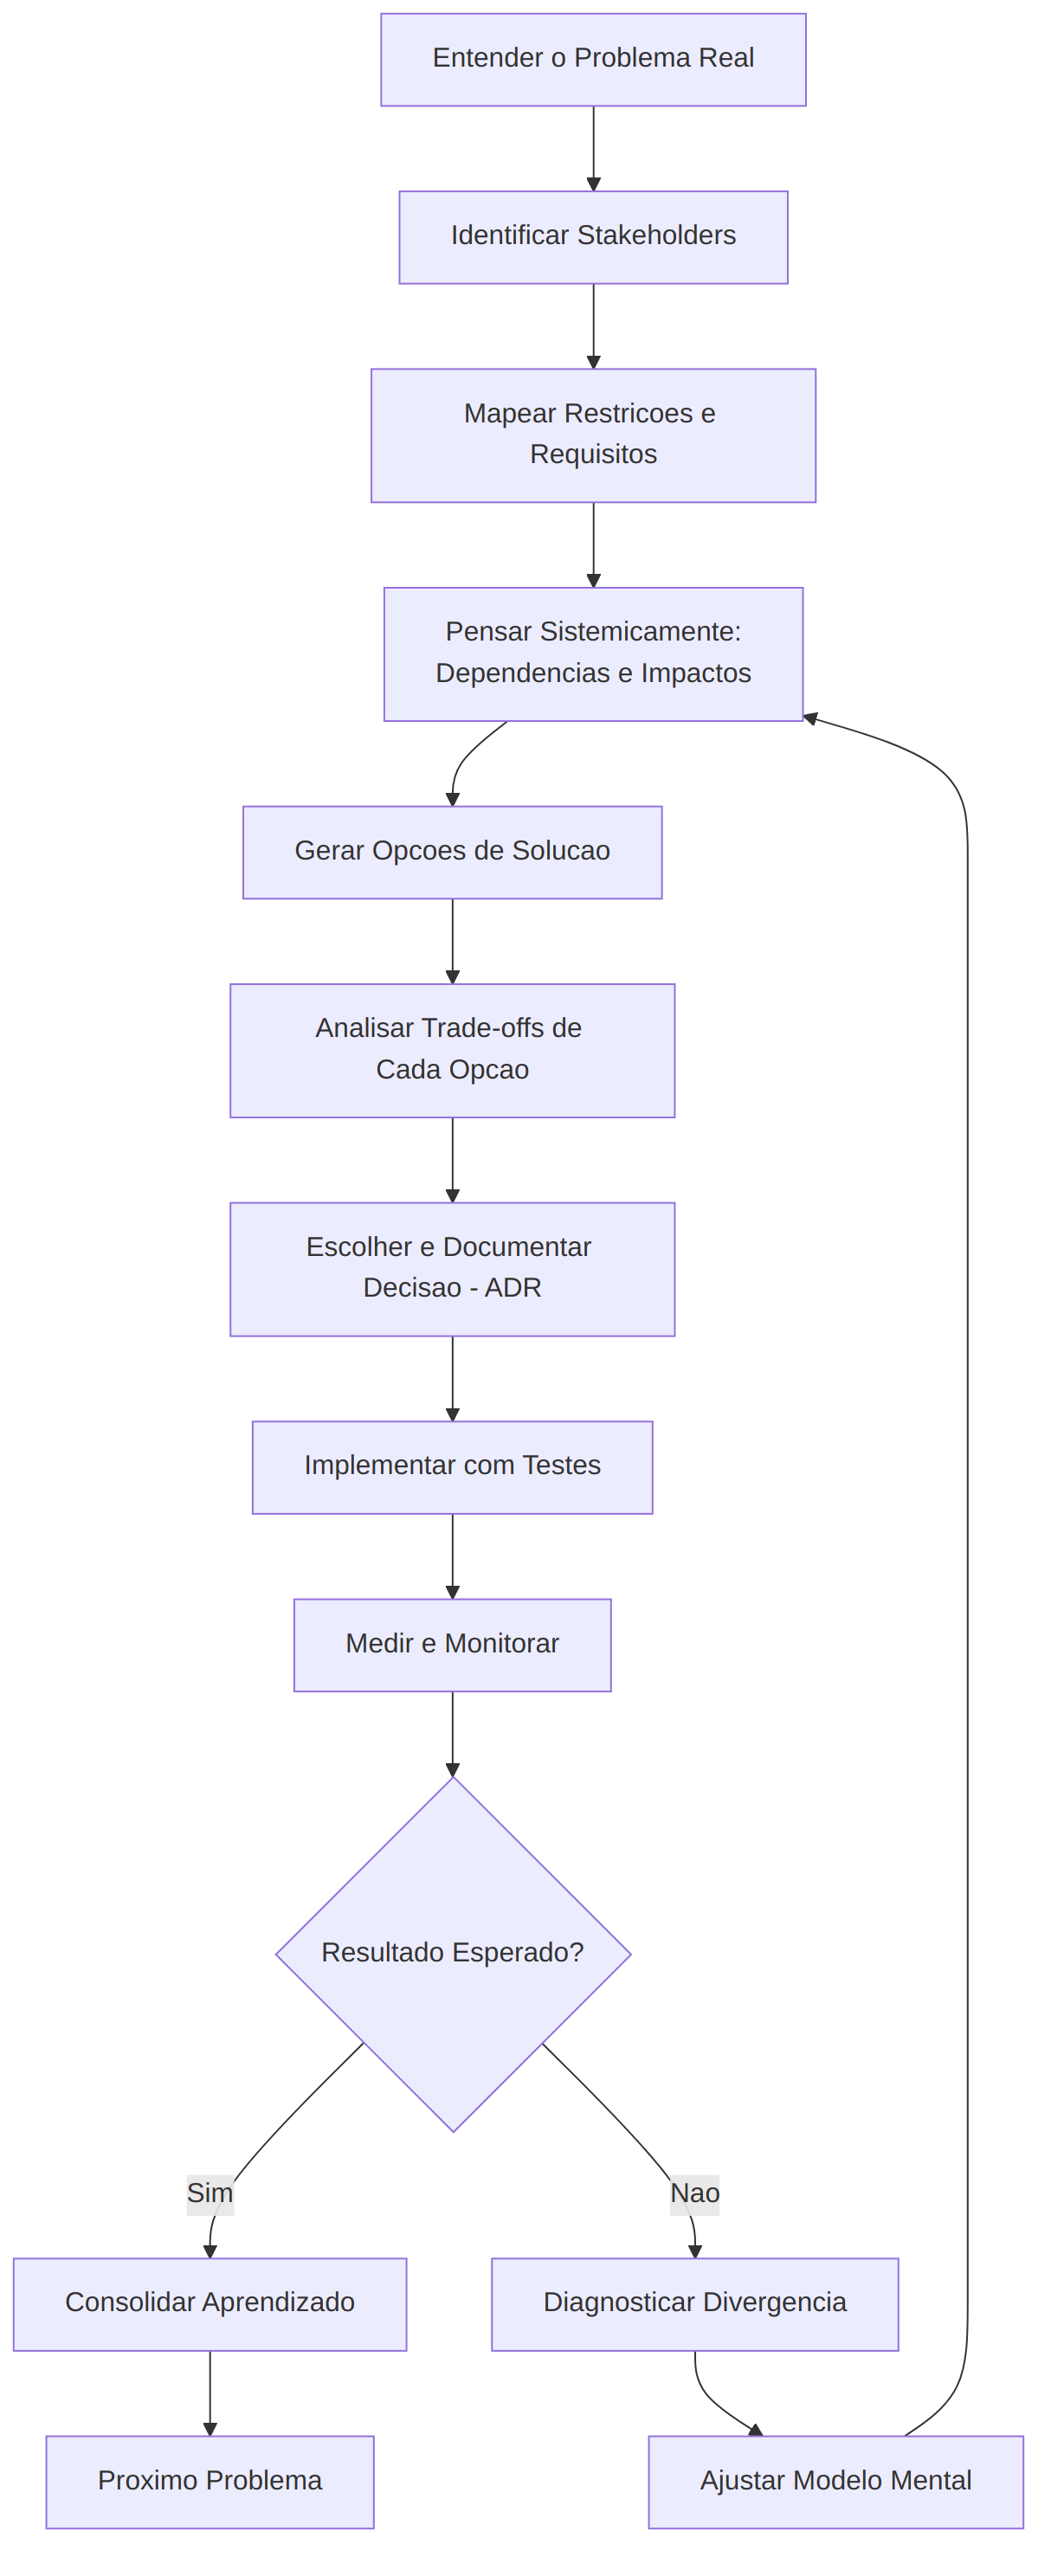
\includegraphics[width=0.85\textwidth]{imagens/00-fundamentos-pensamento-engenharia-05-diagrama-mermaid-o-processo-de-pensamento-do-engenheiro-de-s.png}
    \caption{Diagrama Mermaid: O Processo de Pensamento do Engenheiro de Software}
\end{figure}

Observe que o processo é \textbf{cíclico}, não linear. O resultado da implementação retroalimenta o entendimento do problema, refinando os modelos mentais do engenheiro. Cada iteração torna o engenheiro mais eficaz, não porque ele decorou mais APIs, mas porque seus modelos mentais se tornaram mais precisos.

Este processo também incorpora humildade epistêmica: o reconhecimento explícito de que nosso entendimento inicial pode estar errado, e que o feedback da realidade é mais confiável do que nossas suposições.

\section{Ética e Responsabilidade Profissional}

\subsection{O Poder e o Peso do Código}

Engenheiros de software exercem um poder extraordinário sobre a vida das pessoas, frequentemente sem perceber. O algoritmo de recomendação que você treina influencia o que milhões de pessoas assistem, leem e pensam. O sistema de scoring de crédito que você implementa determina quem recebe um empréstimo e quem não recebe. O software embarcado que você escreve controla sistemas que podem matar se falharem.

Esse poder vem acompanhado de uma responsabilidade proporcional. ``Foi o QA que deveria ter pego'' não é uma desculpa aceitável. ``O product manager pediu para entregar rápido'' não absolve o engenheiro de ter cortado testes de segurança. A responsabilidade profissional do engenheiro não é delegável --- ela é inerente ao ato de escrever código que será executado no mundo real.

\subsection{Casos que Mudaram a Indústria}

\textbf{Therac-25 (1985--1987).} A máquina de radioterapia Therac-25 administrou doses massivas de radiação a pelo menos seis pacientes, causando mortes e ferimentos graves. A causa raiz foi uma combinação de \emph{race conditions} no software, ausência de hardware de segurança redundante (presente em modelos anteriores mas removido porque ``o software cuida disso'') e uma cultura organizacional que descartava relatórios de falha. O caso Therac-25 é ensinado em cursos de engenharia de software no mundo inteiro como o exemplo definitivo de por que validação, testes e humildade são inegociáveis.

\textbf{Boeing 737 MAX (2018--2019).} O sistema MCAS (\emph{Maneuvering Characteristics Augmentation System}) foi projetado para compensar uma característica aerodinâmica resultante da instalação de motores maiores. O software dependia de um \textbf{único} sensor de ângulo de ataque, sem redundância. Quando esse sensor falhava, o MCAS empurrava o nariz do avião para baixo repetidamente, e os pilotos não conseguiam sobrepor o sistema. Dois acidentes --- Lion Air 610 e Ethiopian Airlines 302 --- mataram 346 pessoas. A investigação revelou pressões de cronograma, falhas de comunicação entre engenheiros e gerência, e uma cultura que priorizou custo sobre segurança.

\textbf{Knight Capital Group (2012).} Uma atualização de software implantada incorretamente fez com que o sistema de trading da Knight Capital executasse milhões de operações erráticas no mercado de ações em apenas 45 minutos. O prejuízo de 440 milhões de dólares levou a empresa à falência. A causa foi uma combinação de deploy manual sem rollback automatizado, código legado não removido e ausência de circuit breakers.

Esses casos não são curiosidades históricas. São lembretes de que as decisões que tomamos como engenheiros têm consequências reais, às vezes irreversíveis.

\subsection{Privacidade e Proteção de Dados}

Coletar dados ``porque podemos'' não é ético. A LGPD no Brasil e o GDPR na Europa estabelecem \textbf{mínimos legais} para o tratamento de dados pessoais --- não máximos morais. O engenheiro ético vai além da conformidade legal e pergunta: ``essa coleta de dados é realmente necessária para o serviço que prestamos? Estamos coletando o mínimo necessário? Os dados estão adequadamente protegidos? O que acontece se houver um vazamento?''

O princípio de \textbf{minimização de dados} --- coletar apenas o estritamente necessário para a finalidade declarada --- não é apenas um requisito legal. É uma postura de engenharia: dados que não existem não podem vazar, não precisam ser migrados e não geram custo de armazenamento.

\subsection{Viés Algorítmico e Justiça Computacional}

Sistemas de inteligência artificial treinados com dados enviesados perpetuam e amplificam discriminação. Algoritmos de reconhecimento facial que funcionam bem para homens brancos mas falham para mulheres negras. Sistemas de recrutamento que penalizam currículos de mulheres porque foram treinados com dados históricos de empresas predominantemente masculinas. Modelos de reincidência criminal que atribuem risco maior a réus negros.

O engenheiro de software que constrói ou integra sistemas de IA tem a responsabilidade de questionar os dados de treinamento, testar para viés em subgrupos demográficos e ser transparente sobre as limitações do modelo. ``O algoritmo decidiu'' não é uma resposta aceitável quando o algoritmo perpetua injustiça.

\subsection{Whistleblowing: O Dever Desconfortável}

Quando um engenheiro identifica um problema grave que está sendo deliberadamente ignorado pela gerência --- uma vulnerabilidade de segurança, uma violação de privacidade, um risco à segurança física dos usuários --- ele enfrenta um dilema ético real. Reportar internamente pode ser ignorado. Reportar externamente pode custar o emprego. Mas o silêncio tem um custo que pode ser medido em vidas, dinheiro ou direitos violados.

Não existe resposta fácil para esse dilema. O que existe é o reconhecimento de que o engenheiro profissional não é um executor acrítico de ordens. Ele é um agente moral, com a responsabilidade de levantar a voz quando identifica que algo está errado --- mesmo quando isso é desconfortável.

\section{Conclusão}

Os fundamentos do pensamento de engenharia --- modelos mentais robustos, pensamento sistêmico, análise disciplinada de trade-offs, mentalidade de longo prazo, ciclos de feedback rápidos e responsabilidade ética --- formam a base sobre a qual todo o restante deste livro se constrói. Sem essa mentalidade, ferramentas como inteligência artificial, frameworks e metodologias são martelos procurando pregos: poderosos em potencial, mas destrutivos sem direção.

O engenheiro de software do século XXI não é aquele que escreve mais código, mais rápido. É aquele que pensa com mais clareza, decide com mais rigor e assume a responsabilidade pelo impacto do que constrói. Em uma era em que LLMs podem gerar centenas de linhas de código em segundos, o pensamento se torna o recurso mais escasso --- e mais valioso.

O próximo capítulo avança dos fundamentos conceituais para os modelos concretos: IDEF-0 e RM-ODP, ferramentas de modelagem que permitem transformar o pensamento de engenharia em representações formais, comunicáveis e verificáveis. Veremos como passar da reflexão abstrata à estruturação rigorosa de sistemas.

\section*{Exercícios}

\begin{enumerate}
    \item \textbf{Análise de Trade-offs no Cotidiano.} Identifique um sistema digital que você usa diariamente (ex: aplicativo de banco, rede social, e-commerce). Liste pelo menos 5 trade-offs que os engenheiros provavelmente enfrentaram ao projetá-lo. Para cada trade-off, identifique qual lado foi priorizado e especule sobre as razões.

    \item \textbf{Dívida Técnica Deliberada.} Descreva uma situação real ou hipotética em que assumir dívida técnica deliberadamente seria a decisão \emph{correta}. Explique: (a) qual o atalho, (b) qual o benefício imediato, (c) qual o custo futuro, (d) como você documentaria e gerenciaria essa dívida.

    \item \textbf{Ética e Dados Pessoais.} Você está construindo um sistema de recomendação de conteúdo para uma plataforma educacional voltada a menores de idade. Liste as responsabilidades éticas do engenheiro nesse contexto, considerando: coleta de dados, viés algorítmico, consentimento parental e impacto psicológico das recomendações.

    \item \textbf{Efeitos de Segunda Ordem.} Sua equipe decide migrar de um banco relacional (PostgreSQL) para um banco de documentos (MongoDB) para ``ganhar flexibilidade''. Mapeie pelo menos 5 efeitos de segunda ordem dessa decisão, classificando cada um como positivo, negativo ou neutro.

    \item \textbf{Architecture Decision Record (ADR).} Escreva um ADR completo para uma decisão técnica de um projeto pessoal ou profissional. Inclua: contexto, decisão, alternativas consideradas, consequências positivas e negativas.

    \item \textbf{Pensamento por Primeiros Princípios.} Sua equipe afirma que ``precisamos de microsserviços''. Aplique o pensamento por primeiros princípios: (a) decomponha a afirmação em premissas fundamentais, (b) questione cada premissa, (c) reconstrua o raciocínio a partir das verdades verificáveis. Que conclusão você alcança?

    \item \textbf{Estudo de Caso.} Escolha um dos casos apresentados neste capítulo (Therac-25, Boeing 737 MAX ou Knight Capital). Pesquise detalhes adicionais e escreva uma análise de uma página respondendo: (a) quais decisões de engenharia contribuíram para a falha, (b) quais práticas teriam prevenido ou mitigado o problema, (c) que lições permanentes o caso oferece para engenheiros de software.

    \item \textbf{Mapa de Dependências.} Desenhe um diagrama de dependências para um sistema com o qual você trabalha ou já trabalhou. Identifique: (a) pontos únicos de falha, (b) dependências circulares, (c) componentes com alto fan-in ou fan-out. Proponha pelo menos uma melhoria arquitetural baseada na análise.
\end{enumerate}
